\chapter{Appendice}
\label{cha:appendix}

\section*{Codice SQL per la creazione del database}
\label{appendix:sql}

Il seguente codice SQL definisce la struttura del database a \textbf{costellazione}, illustrata nel Capitolo~\ref{cha:Data_op}.  
Sono incluse la creazione delle tabelle dimensionali e dei fatti, le relazioni tra esse e alcuni record di esempio, utili a comprendere la logica di costruzione del modello.

\begin{lstlisting}[language=SQL, caption={Codice SQL di esempio per la creazione del database}]
-- Creazione del database
CREATE DATABASE CortinaAffluenza;
USE CortinaAffluenza;

-- ==========================
-- TABELLE DIMENSIONALI
-- ==========================

CREATE TABLE Dim_Anno (
    Id_Anno  INT AUTO_INCREMENT PRIMARY KEY ,
    Anno INT NOT NULL
);

CREATE TABLE Dim_Mese (
    Id_Mese INT AUTO_INCREMENT PRIMARY KEY ,
    Nome_Mese VARCHAR(20),
    Numero INT,
    Id_Anno INT,
    FOREIGN KEY (Id_Anno) REFERENCES Dim_Anno(Id_Anno)
);

CREATE TABLE Dim_Settimana (
    Id_Settimana INT AUTO_INCREMENT PRIMARY KEY ,
    Id_Mese INT,
    FOREIGN KEY (Id_Mese) REFERENCES Dim_Mese(Id_Mese)
);

CREATE TABLE Dim_Giorno (
    Id_Giorno INT AUTO_INCREMENT PRIMARY KEY ,
    Data DATE,
    Giorno_Sett VARCHAR(15),
    Is_Holiday BOOLEAN,
    Id_Settimana INT,
    FOREIGN KEY (Id_Settimana) REFERENCES Dim_Settimana(Id_Settimana)
);

CREATE TABLE Dim_Temperatura (
    Id_Temperatura INT AUTO_INCREMENT PRIMARY KEY ,
    Temp_Min DECIMAL(5,2),
    Temp_Media DECIMAL(5,2),
    Temp_Max DECIMAL(5,2)
);

CREATE TABLE Dim_Vento (
    Id_Vento INT AUTO_INCREMENT PRIMARY KEY ,
    Direzione VARCHAR(20),
    Velocita DECIMAL(5,2)
);

CREATE TABLE Dim_CondizioneMeteo (
    Id_CondMeteo INT AUTO_INCREMENT PRIMARY KEY ,
    Tipo_Precipitazione DECIMAL(5,2),
    Id_Temperatura INT,
    Id_Vento INT,
    FOREIGN KEY (Id_Temperatura) REFERENCES Dim_Temperatura(Id_Temperatura),
    FOREIGN KEY (Id_Vento) REFERENCES Dim_Vento(Id_Vento)
);

CREATE TABLE Dim_Stagione (
    Id_Stagione INT AUTO_INCREMENT  PRIMARY KEY ,
    Nome_Stagione VARCHAR(30),
    Data_Inizio DATE,
    Data_Fine DATE
);

CREATE TABLE Dim_TipoSkipass (
    Id_Skipass INT AUTO_INCREMENT PRIMARY KEY,
    Nome_Tipologia VARCHAR(30)
);

CREATE TABLE Dim_AreaSciistica (
    Id_Area INT AUTO_INCREMENT PRIMARY KEY,
    Nome_Area VARCHAR(50)
);

CREATE TABLE Dim_Impianto (
    Id_Impianto INT AUTO_INCREMENT PRIMARY KEY ,
    Nome_Impianto VARCHAR(50),
    Tipo_Impianto VARCHAR(30),
    Id_Area INT,
    FOREIGN KEY (Id_Area) REFERENCES Dim_AreaSciistica(Id_Area)
);

-- ==========================
-- TABELLE DEI FATTI
-- ==========================

CREATE TABLE Fatto_AffluenzaGiornaliera (
    Id_Affluenza INT AUTO_INCREMENT PRIMARY KEY ,
    Id_Giorno INT,
    Id_Impianto INT,
    Id_Skipass INT,
    Id_CondMeteo INT,
    Id_Stagione INT,
    Passaggi_Tot INT,
    FOREIGN KEY (Id_Giorno) REFERENCES Dim_Giorno(Id_Giorno),
    FOREIGN KEY (Id_Impianto) REFERENCES Dim_Impianto(Id_Impianto),
    FOREIGN KEY (Id_Skipass) REFERENCES Dim_TipoSkipass(Id_Skipass),
    FOREIGN KEY (Id_CondMeteo) REFERENCES Dim_CondizioneMeteo(Id_CondMeteo),
    FOREIGN KEY (Id_Stagione) REFERENCES Dim_Stagione(Id_Stagione)
);

CREATE TABLE Fatto_AffluenzaStagionale (
    Id_Affluenza_Stagionale INT AUTO_INCREMENT PRIMARY KEY ,
    Id_Impianto INT,
    Id_Skipass INT,
    Id_Stagione INT,
    Passaggi_Totali INT,
    FOREIGN KEY (Id_Impianto) REFERENCES Dim_Impianto(Id_Impianto),
    FOREIGN KEY (Id_Skipass) REFERENCES Dim_TipoSkipass(Id_Skipass),
    FOREIGN KEY (Id_Stagione) REFERENCES Dim_Stagione(Id_Stagione)
);

-- ==========================
-- INSERIMENTO DATI ESEMPLIFICATIVI
-- ==========================

INSERT INTO Dim_Anno (Anno) VALUES (2023), (2024);

INSERT INTO Dim_Mese (Nome_Mese, Numero, Id_Anno)
VALUES ('Gennaio', 1, 1), ('Febbraio', 2, 1);

INSERT INTO Dim_Settimana (Id_Mese) VALUES (1), (2);

INSERT INTO Dim_Giorno (Data, Giorno_Sett, Is_Holiday, Id_Settimana)
VALUES ('2023-01-10', 'Martedi', FALSE, 1),
       ('2023-02-15', 'Mercoledi', FALSE, 2);

INSERT INTO Dim_Temperatura (Temp_Min, Temp_Media, Temp_Max)
VALUES (-10.5, -6.2, -2.1);

INSERT INTO Dim_Vento (Direzione, Velocita)
VALUES ('Nord', 15.3);

INSERT INTO Dim_CondizioneMeteo (Tipo_Precipitazione, Id_Temperatura, Id_Vento)
VALUES (2.0, 1, 1);

INSERT INTO Dim_Stagione (Nome_Stagione, Data_Inizio, Data_Fine)
VALUES ('2023/2024', '2023-12-01', '2024-04-15');

INSERT INTO Dim_TipoSkipass (Nome_Tipologia)
VALUES ('Dolomiti Superski'), ('Di Valle');

INSERT INTO Dim_AreaSciistica (Nome_Area)
VALUES ('Tofana');

INSERT INTO Dim_Impianto (Nome_Impianto, Tipo_Impianto, Id_Area)
VALUES ('Freccia nel Cielo', 'Funivia', 1),
       ('Tofana Express', 'Seggiovia', 1);

INSERT INTO Fatto_AffluenzaGiornaliera
(Id_Giorno, Id_Impianto, Id_Skipass, Id_CondMeteo, Id_Stagione, Passaggi_Tot)
VALUES (1, 1, 1, 1, 1, 1200),
       (2, 2, 2, 1, 1, 850);

INSERT INTO Fatto_AffluenzaStagionale
(Id_Impianto, Id_Skipass, Id_Stagione, Passaggi_Totali)
VALUES (1, 1, 1, 180000),
       (2, 2, 1, 95000);

\end{lstlisting}


\section*{Campi Calcolati}
Di seguito è riportato l’elenco completo dei campi calcolati utilizzati nelle analisi sviluppate su \textit{Tableau}.  
Tali campi hanno permesso di creare variabili dinamiche e derivate, in particolare per il calcolo della temperatura percepita e per la gestione dei parametri meteorologici.

\begin{lstlisting}[language=SQL, caption={Campo calcolato: Temperatura Base}]
IF [TipoTemperatura] = "Minima" THEN
    [Temp Min (C)]
ELSE
    [Temp Media (C)]
END
\end{lstlisting} \label{appendix:Temp_Base}


\begin{lstlisting}[language=SQL, caption={Campo calcolato: Temperatura Percepita (Wind Chill)}]
IF ISNULL([Temperatura Base]) THEN
    NULL
ELSEIF [Temperatura Base] <= 10 
   AND ([Velocita vento  (m/s)] * 3.6) > 4.8 THEN
    ROUND(
        13.12
      + 0.6215 * [Temperatura Base]
      - 11.37 * POWER(([Velocita vento  (m/s)] * 3.6), 0.16)
      + 0.3965 * [Temperatura Base] * POWER(([Velocita vento  (m/s)] * 3.6), 0.16),
    1)
ELSE
    [Temperatura Base]
END
\end{lstlisting}\label{appendix:Temp_percepita}

\begin{lstlisting}[language=SQL, caption={Campo calcolato: Selettore Tipologia di Skipass}]
IF [Selezione Skipass] = "DS" THEN 
    [Pass. DS]

ELSEIF [Selezione Skipass] = "Valle" THEN 
    [Pass. Valle]

ELSE 
    [Passaggi Tot]
END
\end{lstlisting}\label{appendix:tipo_skipass}


\noindent
Nelle sezioni successive sono riportate alcune visualizzazioni supplementari e di dettaglio, non incluse nel corpo principale della tesi ma rilevanti per il completamento dell’analisi.

\section*{Analisi 1}

\subsection*{Specifica Giorno}
Esempio della vista dettagliata di un singolo giorno, che consente di analizzare i valori puntuali dei passaggi registrati nella data selezionata.

\begin{figure}[h]
    \centering
    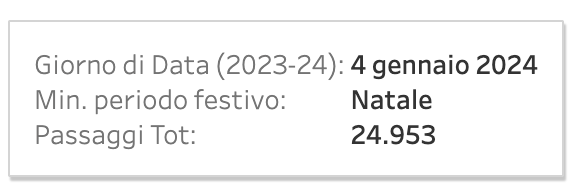
\includegraphics[width=0.5\linewidth]{images/Tableau/Studio_1/4_gennaio.png}
    \caption{Specifica del Giorno}
    \label{fig:spec_giorno}
\end{figure}

\subsection*{Grafico passaggi totali per Settimana}
Versione aggregata del grafico principale dell’analisi 1, ottenuta tramite operazione di \textbf{Roll-Up} sulla gerarchia temporale, che mostra i passaggi totali per settimana.

\begin{figure}[htbp]
    \centering
    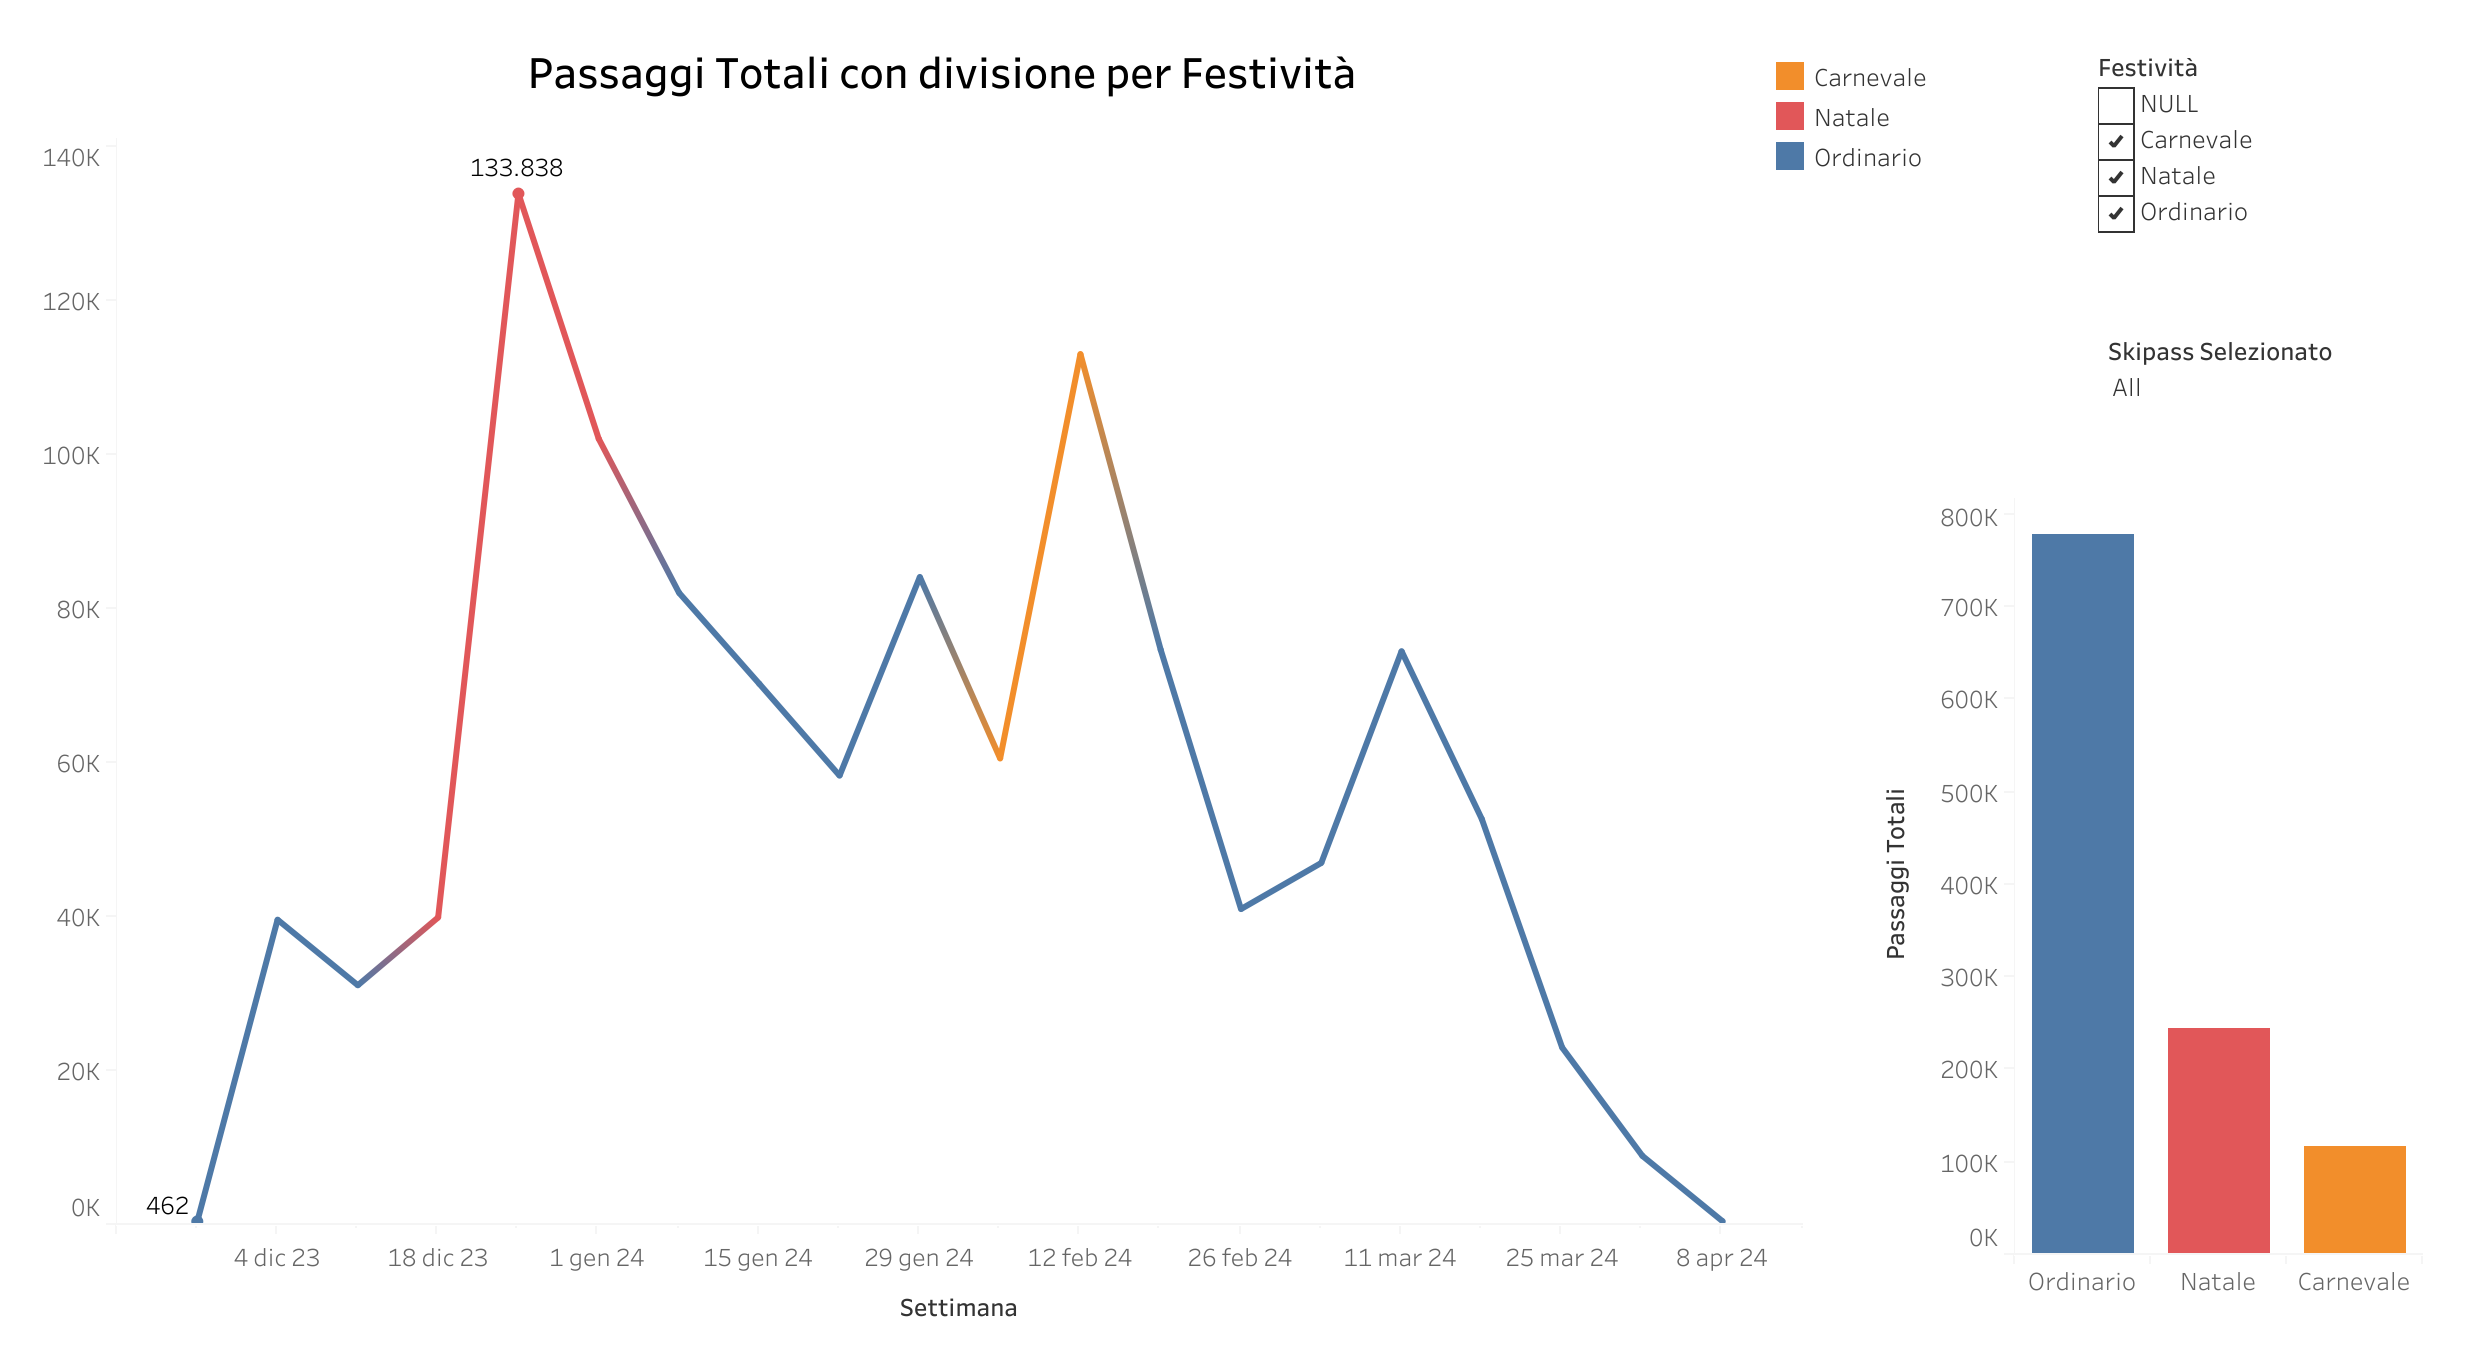
\includegraphics[width=0.95\textwidth]{images/Tableau/Studio_1/Passaggi Totali Settimana.png}
    \caption{Andamento settimanale dei passaggi totali nella stagione 2023–24, suddivisi per periodo festivo.}
    \label{fig:passaggi_tot_settimana}
\end{figure}

\subsection*{Grafico passaggi totali per giorno - Natale}
Vista alternativa del grafico principale della prima analisi, con filtro per l’esclusione del periodo natalizio.  
Questa impostazione evidenzia la costanza del periodo carnevalesco e la sua stabilità nel corso della stagione.

\begin{figure}[htbp]
    \centering
    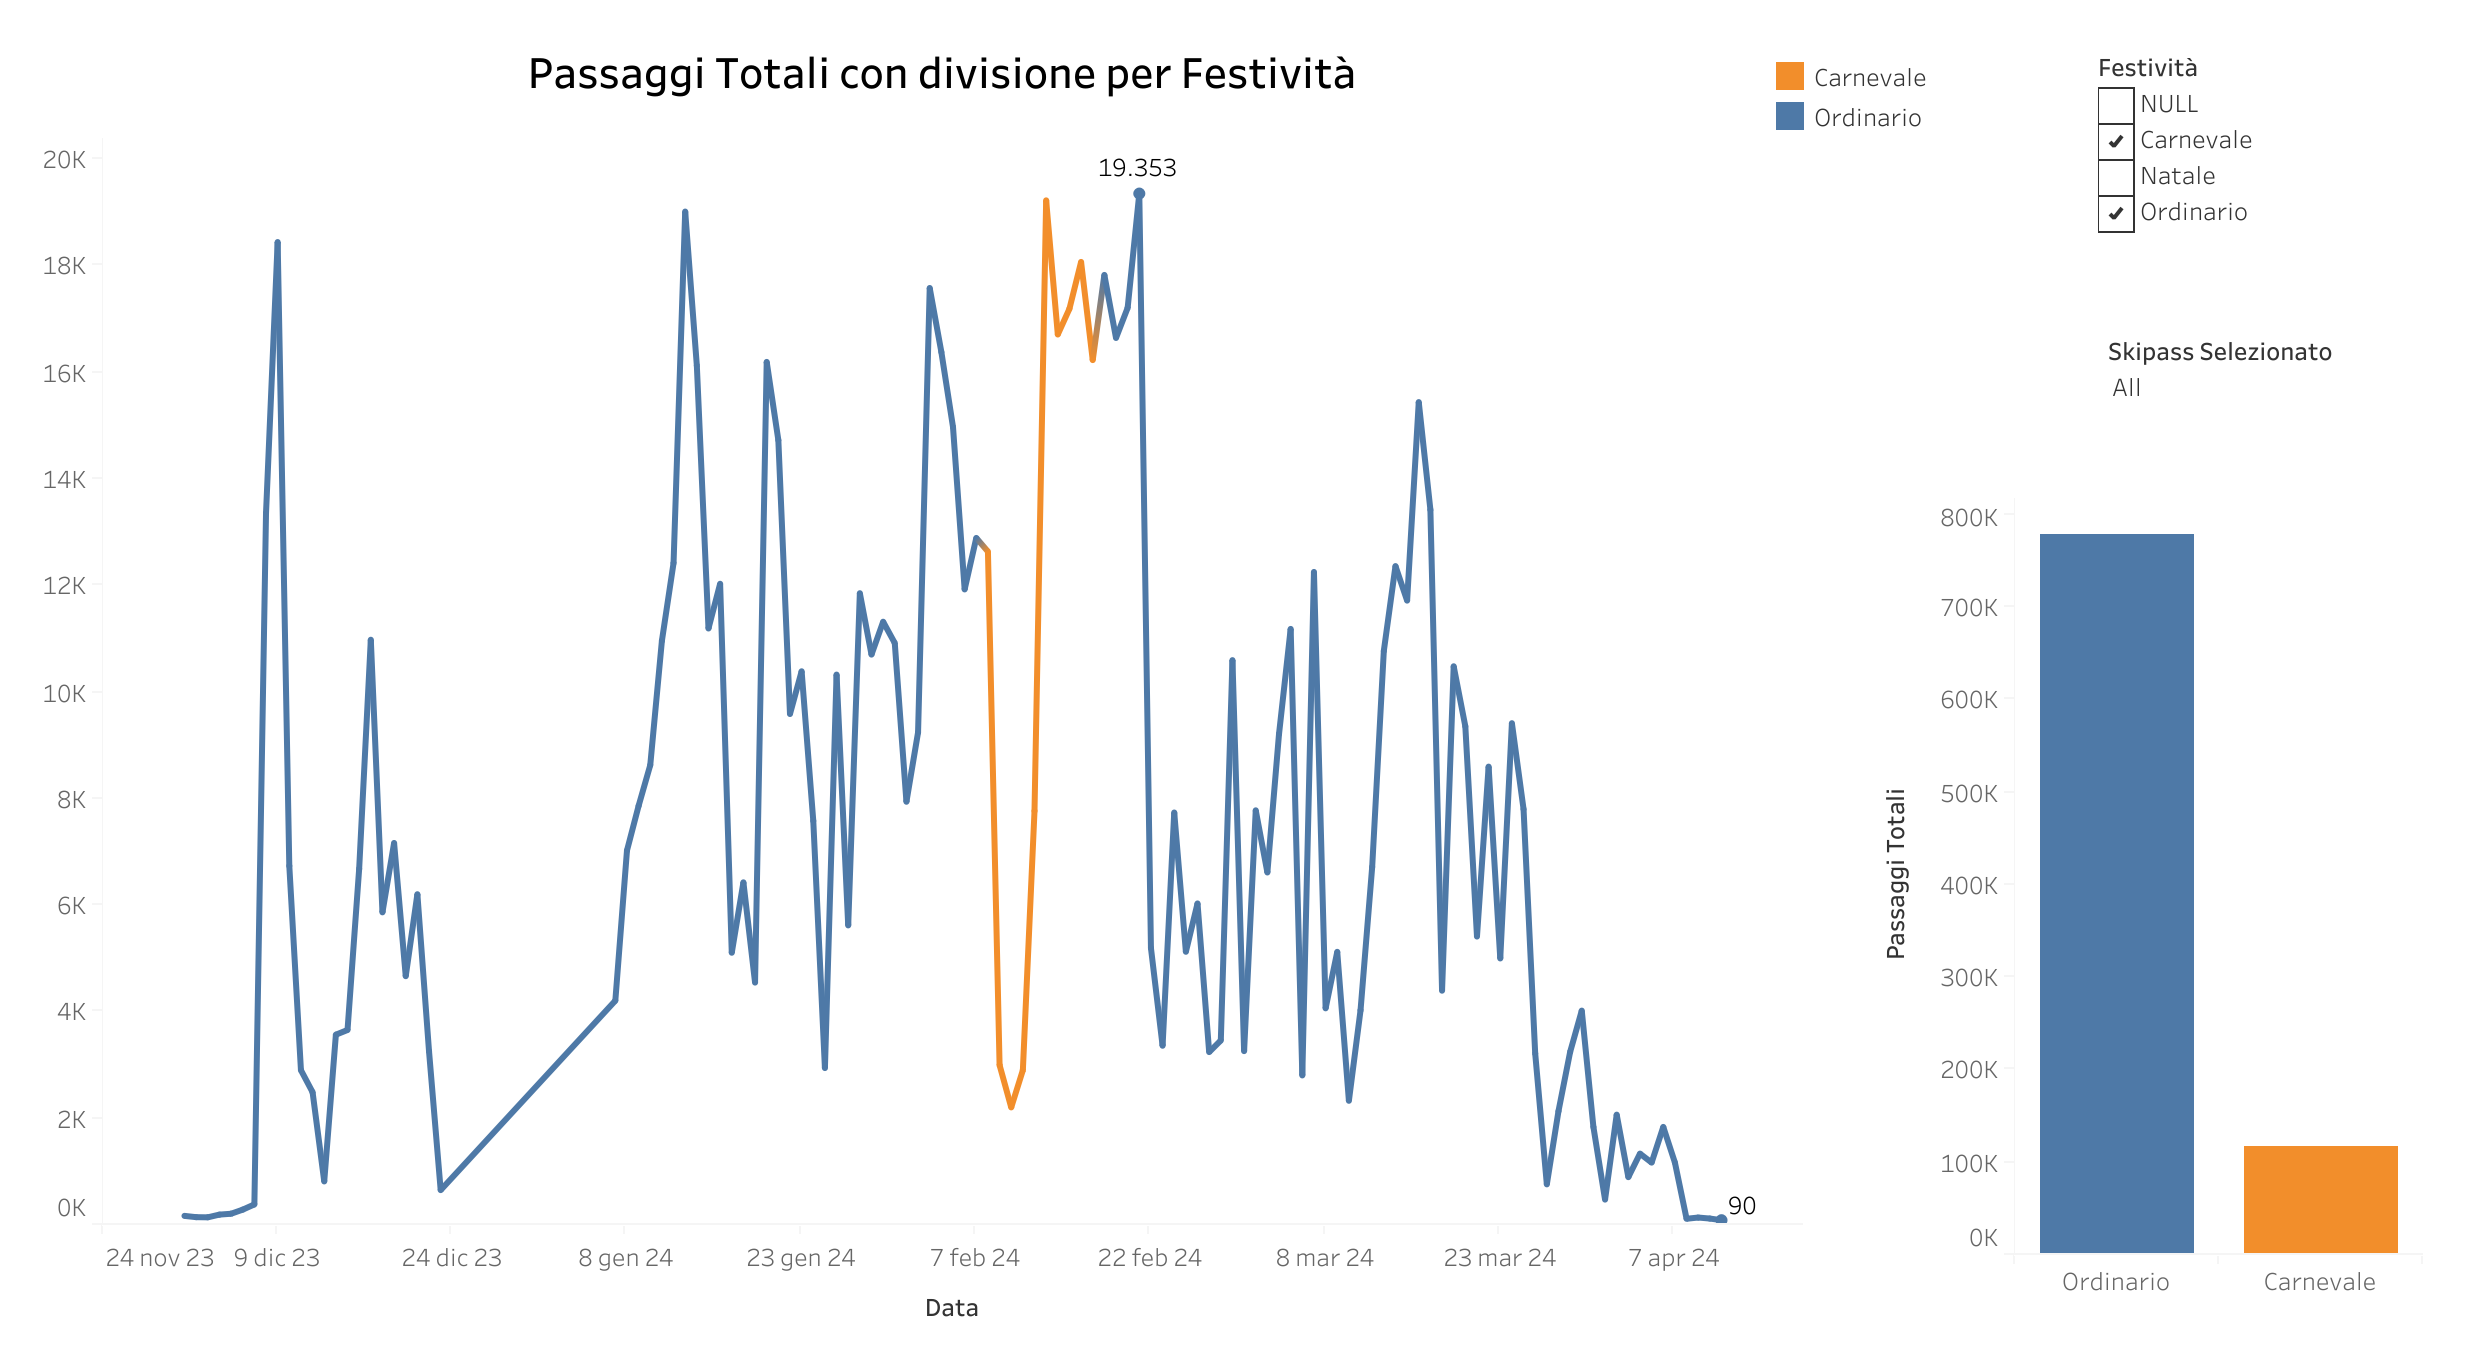
\includegraphics[width=0.9\textwidth]{images/Tableau/Studio_1/Passaggi Totali_noNatale.png}
    \caption{Andamento stagionale dei Passaggi totali con esclusione del periodo Natalizio}
    \label{fig:passaggi_tot_noNatale}
\end{figure}


\section*{Analisi 2}
La seguente dashboard, descritta nel Capitolo~\ref{sec:analisi2}, mostra l’andamento dei passaggi giornalieri per giorno della settimana.  
In questa vista è stato incluso anche il \textbf{martedì} attraverso il filtro “\textbf{Selezione Giorno}”, per evidenziare la sua rilevanza in termini di affluenza.

\begin{figure}[htbp]
    \centering
    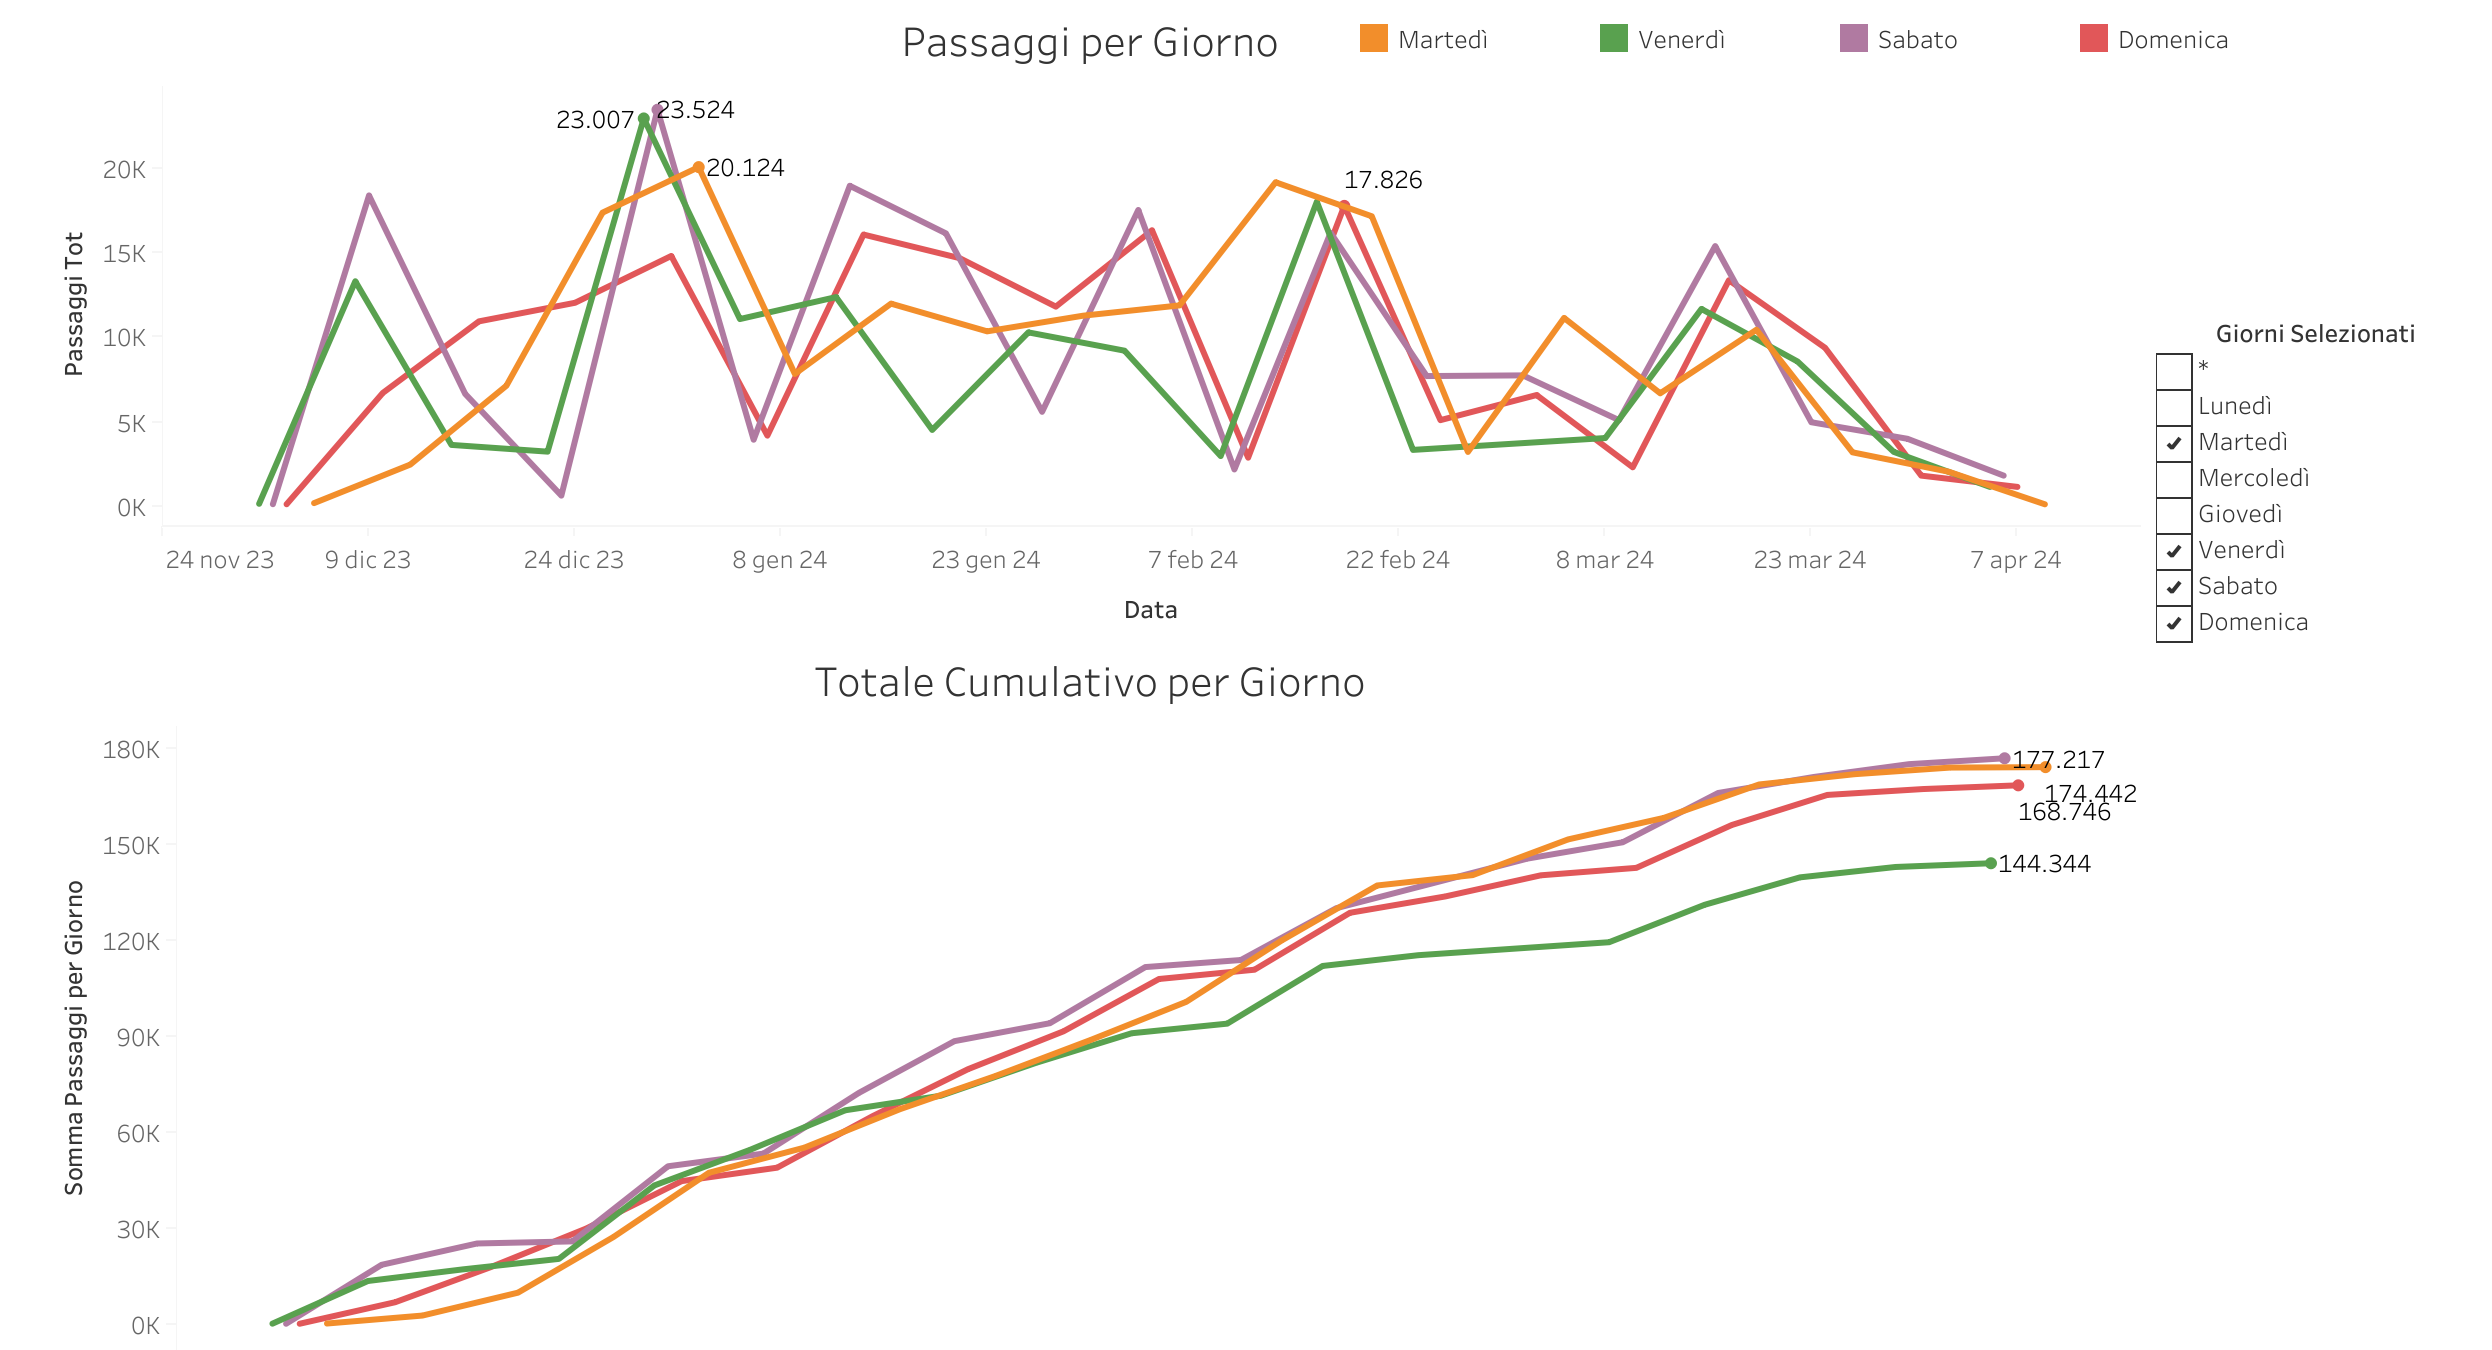
\includegraphics[width=0.9\textwidth]{images/Tableau/Studio_2/Dash_Tuesday.png}
    \caption{Dashboard per passaggi settimanali con totale cumulativo con l'inclusione del Martedì.}
    \label{fig:dash_tuesday}
\end{figure}


\section*{Analisi 4}
Di seguito vengono riportati i campi calcolati e le dashboard utilizzate per l’analisi sull’impatto delle precipitazioni nevose in relazione alle diverse tipologie di skipass.  
La figura seguente mostra l’esempio riferito agli utenti in possesso dello \textbf{skipass di Valle}.




\begin{figure}[htbp]
    \centering
    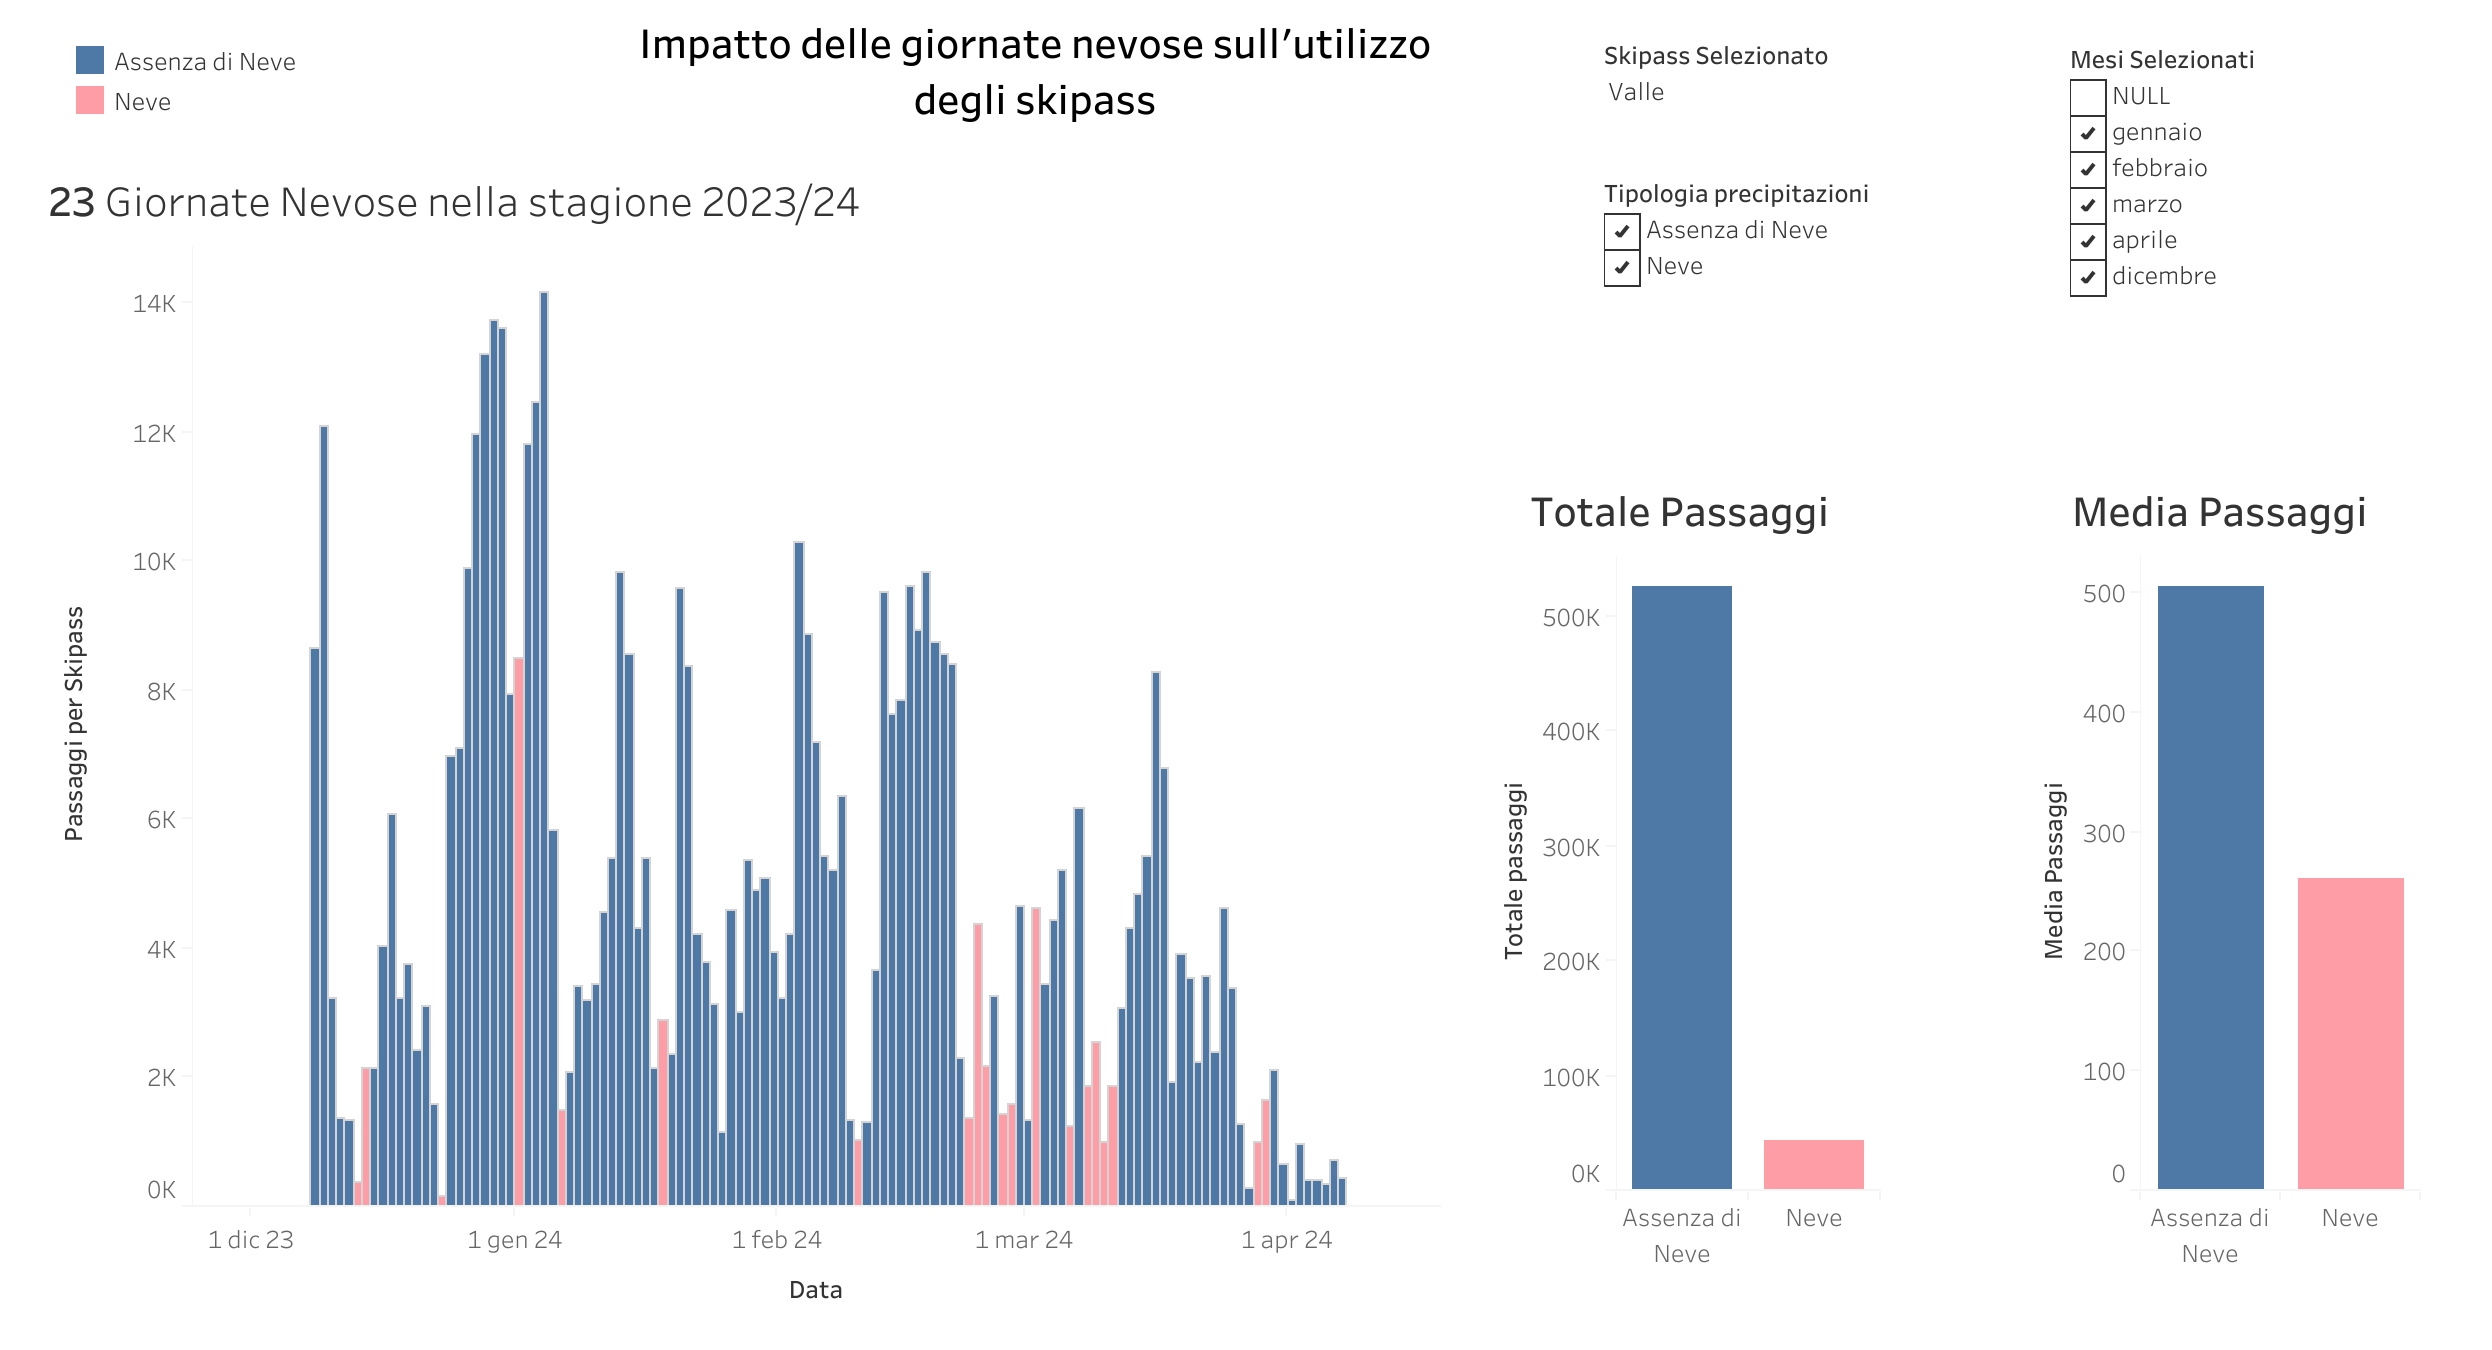
\includegraphics[width=0.95\textwidth]{images/Tableau/Studio_4/Impatto_Neve_valle.png}
    \caption{Dashboard Impatto giornate sull'utilizzo degli Skipass, vista Skipass di Valle}
    \label{fig:Impatto_neve_Valle}
\end{figure}

%\section*{Vista complessiva}
%--Di seguito viene riportata un immagine contenente le 4 dashboard raffigurate nel quarto capitolo dell'elaborato in uan vista unica.

\section*{Vista Completa}
Di seguito viene riportato un \textbf{QR-Code} che rimanda alla pagina dedicata su \textit{Tableau Public}, dove sono raccolte tutte le visualizzazioni interattive e i grafici realizzati per questo elaborato.
L’accesso alla piattaforma consente di esplorare dinamicamente le dashboard, modificare i filtri e approfondire in autonomia le analisi presentate nel capitolo~4\ref{cha:Analisi}.\\

Nella pagina successiva è inoltre inserita un’immagine riepilogativa che mostra le quattro dashboard principali dello studio, offrendo una visione d’insieme delle soluzioni analitiche sviluppate e del loro contributo all’interpretazione dei dati.

\vspace{3cm}
\begin{figure}[htbp]
    \centering
    % Larghezza consigliata: 0.35-0.45 della pagina
    
\includegraphics[width=0.35\textwidth]{images/qr/qr_tableau.png}
    \caption{Visualizzazione Interattiva - Tableau Public}
    \label{fig:qr_tableau}
\end{figure}


\begin{landscape}

\vspace{1em}

\begin{figure}[h]
    \centering
    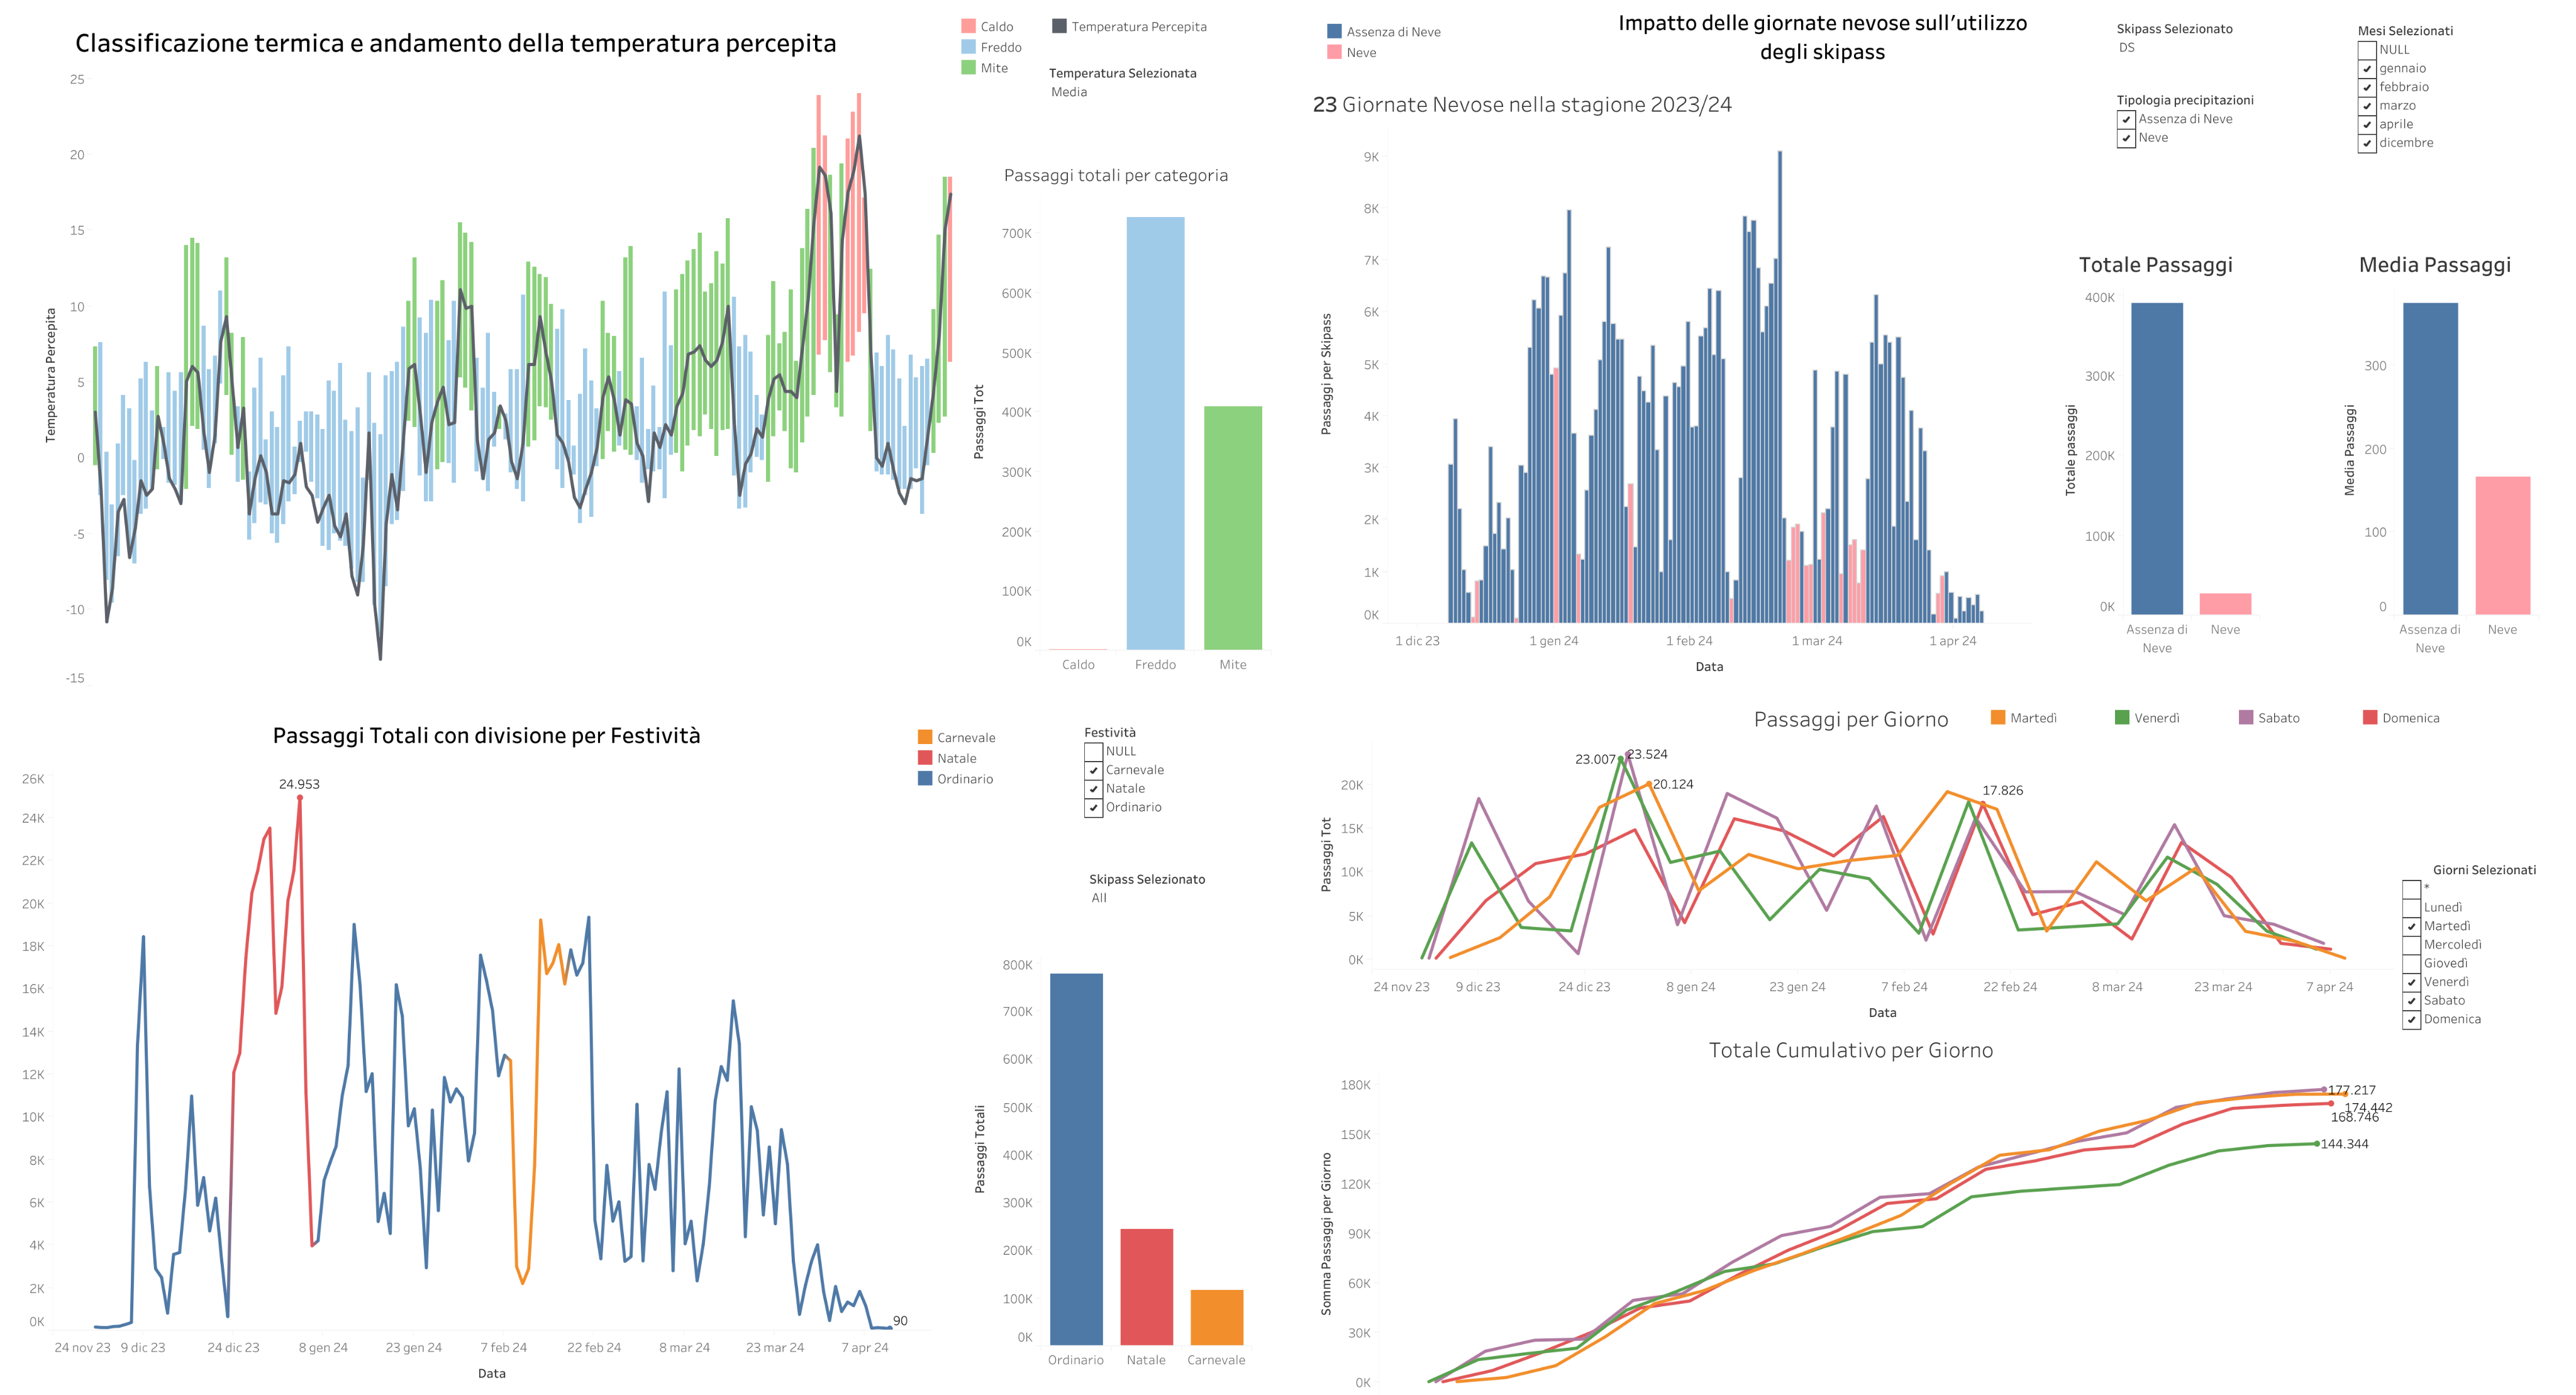
\includegraphics[width=0.95
    \linewidth, height=0.90\textheight]{images/Tableau/dashboard_complessiva.png}
    \caption{Dashboard riunite in un'unica immagine}
    \label{fig:vista_completa}
\end{figure}
\end{landscape}



